\subsubsection{Tiling Technique}

The \definition{Tiling Technique}, also known as \textbf{\emph{blocked matrix multiplication}} or \textbf{\emph{tiling}}, is a strategy to \textbf{enhance the performance of matrix computations by optimizing memory access patterns}. It leverages shared memory in CUDA to reduce the number of global memory accesses, improving efficiency and throughput. A lot of parallel algorithms adopt the tiling technique.

\highspace
\begin{flushleft}
    \textcolor{Green3}{\faIcon{question-circle} \textbf{What is Tiling?}}
\end{flushleft}
Tiling can be thought of as the \textbf{process of breaking a large matrix into smaller sub-matrices} (called \emph{tiles} or blocks) \textbf{that can fit into faster}, \textbf{limited shared memory}. The \underline{main goal} of tiling is to:
\begin{itemize}
    \item \textbf{Minimize} slower \textbf{global memory accesses};
    \item \textbf{Maximize} the \textbf{use of faster shared memory}.
\end{itemize}
Instead of a large matrix, we can think of the global memory contents as tiles and focus the computation of CUDA threads on one or a small number of tiles at a time.

\highspace
\begin{flushleft}
    \textcolor{Green3}{\faIcon{book} \textbf{Great analogy to understand the basic concept of Tiling}}
\end{flushleft}
Reducing the number of vehicles in a congested traffic system can significantly improve the delays experienced by all vehicles. This is analogous to carpooling for commuters. We can image:
\begin{itemize}
    \item \textbf{Drivers}: represent \emph{threads accessing their memory data operands}.
    \item \textbf{Cars}: represent \emph{memory access requests}.
\end{itemize}
Just as carpooling reduces the number of cars on the road, tiling reduces the number of global memory accesses by loading data into shared memory. The result is a reduction in traffic (memory access requests) and an obvious improvement in overall efficiency.

\highspace
Unfortunately, just like in real life, there are some problems. For example, there are the \textbf{challenges of carpooling}. In fact, some carpools are easier to organize than others because the participants need to have similar work schedules. So certain vehicles may be more suitable for carpooling. However, other \textbf{commuters may have different needs}, \textbf{so the number of carpools may increase and there is a risk of increasing traffic again}.

\highspace
Similar challenges exist in tiling calculations. Some computations may be easier to tile based on data access patterns and the nature of the computation. \textbf{Organizing data and computations efficiently to fit into tiles may be more challenging for certain algorithms}. So what is the \textbf{general euristic to adopt in order to use the tiling technique} or not? In general, it is:
\begin{itemize}
    \item[\textcolor{Green3}{\faIcon{check}}] \textbf{\textcolor{Green3}{\textbf{Good}} to use} tiling when people have similar schedule. In computing, is good \textbf{when threads have \emph{similar access timing}}.

    \item[\textcolor{Red2}{\faIcon{times}}] \textbf{\textcolor{Red2}{\textbf{Bad}} to use} tiling when people have very different schedule. In computing, is bad \textbf{when threads have very \emph{different timing}}.
\end{itemize}
But synchronization is also important. Just as workers' schedules must be aligned for effective carpooling, \textbf{threads} in parallel computing \textbf{must be synchronized} for efficient execution. Efficient data access and memory usage depend on synchronized operations to reduce latency and improve performance. The following figure shows synchronization between multiple threads.

\begin{figure}[!htp]
    \centering
    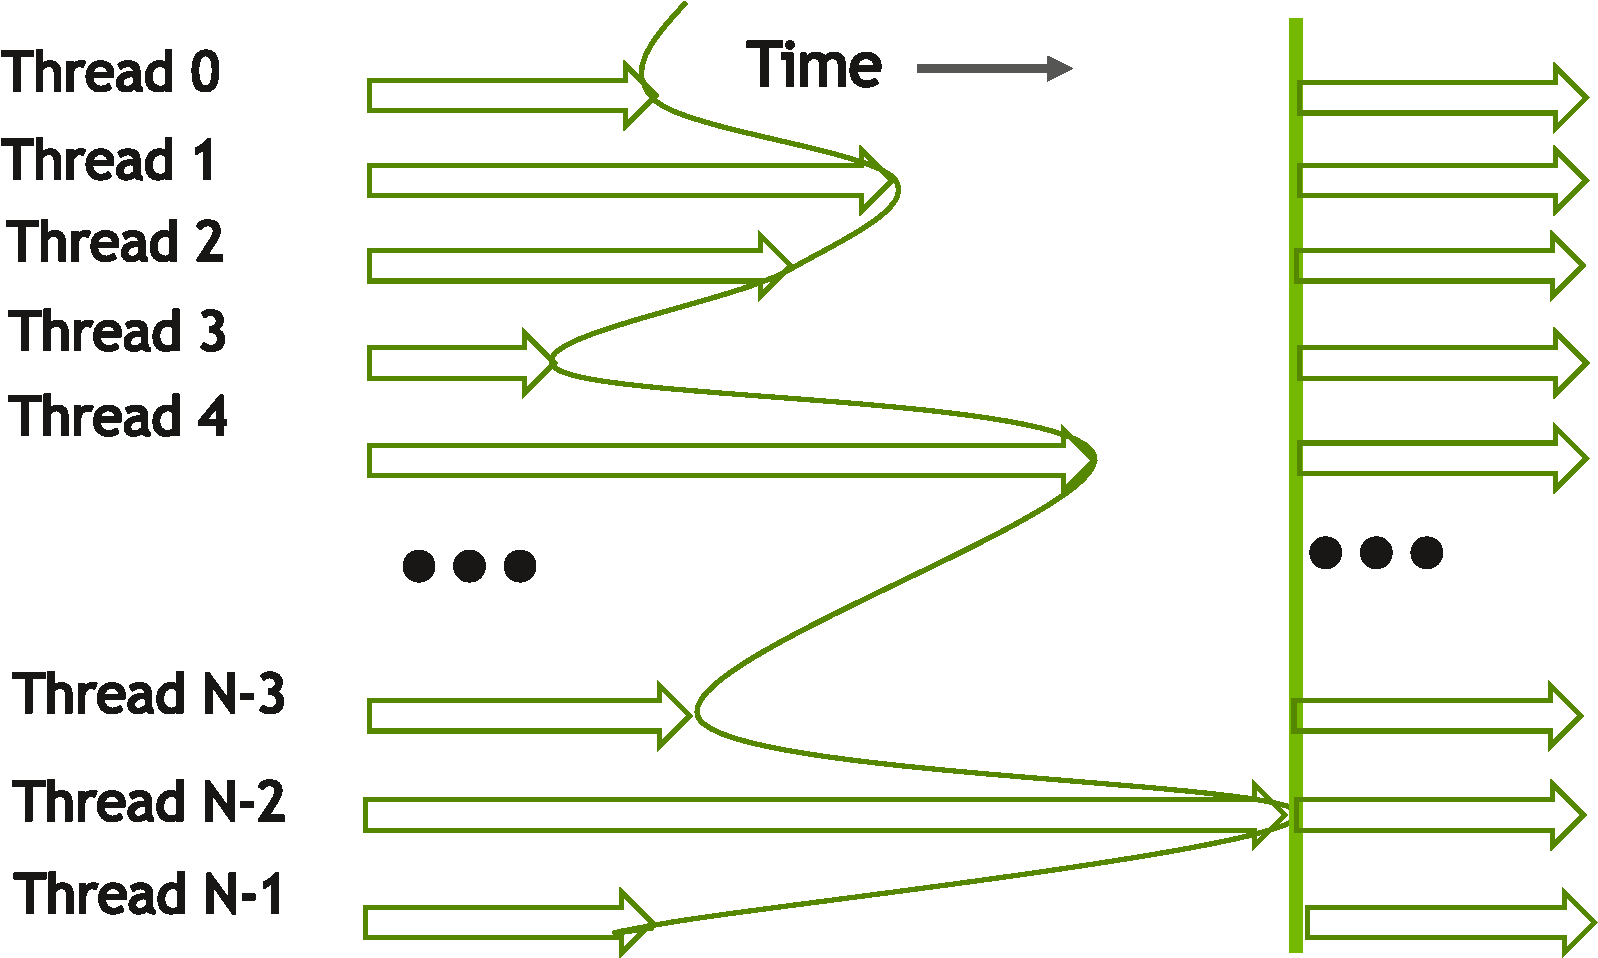
\includegraphics[width=.8\textwidth]{img/cuda-tiling-1.pdf}
    \caption{Barrier Synchronization for Tiling.}
\end{figure}

\noindent
On the left are multiple threads (\texttt{Thread 0}, \texttt{Thread 1}, \texttt{Thread 2}, \dots, \texttt{Thread N-1}) progressing over time. The wave represents when each thread reaches its barrier on the code; at that point, the thread must wait until all threads have arrived before it can continue. This ensures that all threads are synchronized at certain points during execution. Execution of all threads resumes when the last thread (in the picture, \texttt{Thread N-2}) reaches the barrier.

\highspace
\textbf{Synchronization is fundamental in the tiling technique} because it \textbf{ensures that all threads have their share of data loaded into shared memory and are ready to proceed before they perform any computations}. After the computation, they use another synchronization barrier to ensure that all threads have completed their work before moving to the next tile.

\newpage

\begin{flushleft}
    \textcolor{Green3}{\faIcon{tools} \textbf{Summary - How it works}}
\end{flushleft}
\begin{enumerate}
    \item \important{Identify a Tile}. Determine a section of global memory content that multiple threads will access. Dividing the workload into smaller tiles allows for efficient memory access and utilization of shared memory.
    \item \important{Load the Tile}. Transfer the tile from global memory to on-chip memory (shared memory). Loading data into shared memory reduces the latency associated with accessing global memory.
    \item \important{Barrier Synchronization}. Ensures that all threads are ready to begin the computation phase. It also ensures that all threads have the necessary data before starting the computation.
    \item \important{Access Data}. Multiple threads access their data from the on-chip memory. Threads perform computations using the data stored in shared memory, benefiting from its faster access time.
    \item \important{Barrier Synchronization}. Ensure all threads have completed the current phase (computations).
    \item \important{Next Tile}. Move on to the next tile and repeat the process.
\end{enumerate}

\highspace
\begin{flushleft}
    \textcolor{Green3}{\faIcon{check} \textbf{Advantages}}
\end{flushleft}
\begin{itemize}
    \item[\textcolor{Green3}{\faIcon{check}}] \textbf{Improved Memory Access Patterns}. By loading data into shared memory, the number of global memory accesses is reduced, leading to better performance.
    \item[\textcolor{Green3}{\faIcon{check}}] \textbf{Higher Computational Throughput}. Tiling helps achieve higher computational throughput by leveraging the faster shared memory.
\end{itemize}
